\documentclass[a4paper,12pt]{extarticle}
\usepackage{graphicx}
\usepackage{tikz}
\usepackage{hyperref}
\setcounter{tocdepth}{3}
\usetikzlibrary{matrix,shapes,arrows,positioning,chains}
\tikzstyle{normal} = [ anchor=center,
		text width=10em, align=center,
		top color=white, line width=0mm,
		inner sep=1ex]
\tikzstyle{rect} = [shape=rectangle, rounded corners,
		draw, anchor=center,
		text width=10em, align=center,
		inner sep=1ex]

\begin{document}
	\title{Assembler, Linker \& Loader}
	\author{Abhinav Hinger, Apurva N. Saraogi, Daman Tekchandani}
	\maketitle
	\pagebreak
	\tableofcontents
	\pagebreak
	\section{Introduction}
This document is in with the reference to the project given in CS-244(System Programming Lab) course under the guidance of Prof. Santosh Biswas on Assembler, Linker, Loader and it's working for a programming language.\newline\newline
A computer will not understand any program written in a language, other than its
machine language. This document covers how a normal source code is loaded into the memory. It is done in various steps. Below is the flow chart showing exection of a source code.\newline
		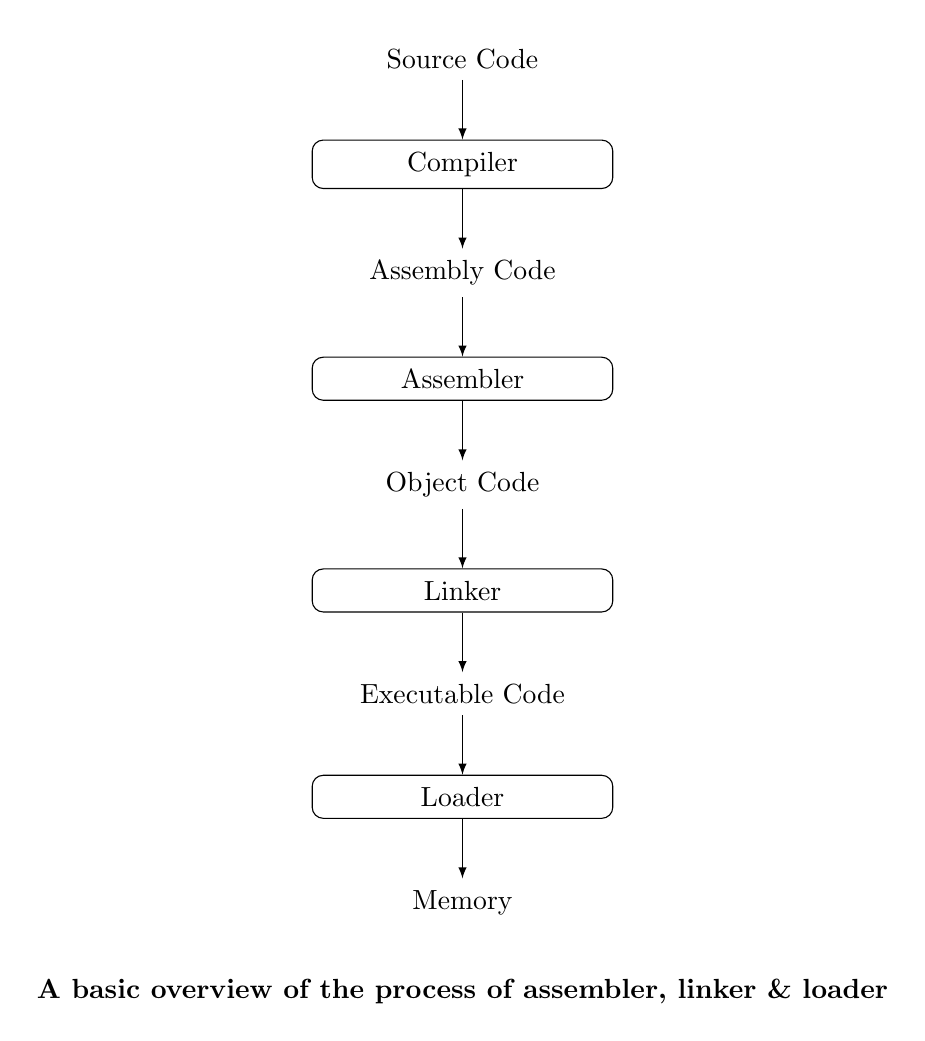
\begin{tikzpicture}
	\matrix (m)[matrix of nodes, column sep = 3em, row sep=5ex]{
		|[normal]|Source Code\\
		|[rect]|Compiler		\\
		|[normal]|Assembly Code		\\
		|[rect]|Assembler		\\
		|[normal]|Object Code		\\
		|[rect]|Linker		\\
		|[normal]|Executable Code		\\
		|[rect]|Loader		\\
		|[normal]|Memory \\
	};
	\path [>=latex,->] (m-1-1) edge (m-2-1);
	\path [>=latex,->] (m-2-1) edge (m-3-1);
	\path [>=latex,->] (m-3-1) edge (m-4-1);
	\path [>=latex,->] (m-4-1) edge (m-5-1);
	\path [>=latex,->] (m-5-1) edge (m-6-1);
	\path [>=latex,->] (m-6-1) edge (m-7-1);
	\path [>=latex,->] (m-7-1) edge (m-8-1);
	\path [>=latex,->] (m-8-1) edge (m-9-1);
	
	\node[align=center,font=\bfseries, yshift=-2em] (title) 
	at (current bounding box.south)
	{A basic overview of the process of assembler, linker \& loader};
	\end{tikzpicture}
	\newline
	\newline
	The programs written in other languages must be translated into
	the machine language. Such translation is performed with the help of software. A program which translates an assembly language program into a machine language
	program is called an assembler.\newline
	In high level languages, some built in header files or libraries are stored. These
	libraries are predefined and these contain basic functions which are essential for executing
	the program. These functions are linked to the libraries by a program called
	Linker. Usually a longer program is divided into smaller subprograms called modules.
	And these modules must be combined to execute the program. The process of
	combining the modules is done by the linker.\newline
	Loader is a program that loads machine codes of a program into the system memory.In
	Computing, a loaderis the part of an Operating System that is responsible
	for loading programs. It is one of the essential stages in the process of starting a
	program. Because it places programs into memory and prepares them for execution.	
	\pagebreak
	\section{Terminologies used \& their details}
	\subsection{Assembly Language}
	Let’s try to understand a assembly language with a simple Example. This will give
	us an insight to the underlying algorithms and data structures which is explained
	later in this \hyperref[sec:assembler]{section}.
	Assembly language program (8085 microprocessor) to add two 8 bit numbers.
	Problem - Write an assembly language program to add two 8 bit numbers stored at
	address 2050 and address 2051 in 8085 microprocessor. Starting address of program
	is taken as 2000.\newline
	Algorithm
	\begin{enumerate}
		\item First add contents of memory location 2050 and 2051 using “ADD” instruction
		and storing at 3050.
		\item The carry generated is recovered using “ADC” command and is stored at memory
		location 3051.
	\end{enumerate}
	Explanation
	\begin{enumerate}
		\item LHLD 2050 moves the contents of 2050 memory location (3B) in L register
		and contents of 2051 memory location (F9) in H register.
		\item MOV A, L copies contents of L register (3B) to A (Accumulator).
		\item ADD H adds contents of A (Accumulator) and H register (F9). The result is
		stored in A itself. For all arithmetic instructions A is by default an operand
		and A stores the result as well.
		\item MOV L, A copies contents of A (34) to L.
		\item MVI A 00 moves immediate data (i.e., 00) to A.
		\item ADC A adds contents of A(00), contents of register specified (i.e A) and carry
		(1) As ADC is also an arithmetic operation, A is by default an operand and
		\newline A stores the result as well.
		\item MOV H, A copies contents of A (01) to H.
		\item SHLD 3050 moves the contents of L register (34) in 3050 memory location and
		contents of H register (01) in 3051 memory location.
		\item HLT stops executing the program and halts any further execution.
	\end{enumerate}
	
	Consider another problem which might further clear the understanding of assembly
	language programming.
	Add the contents of memory locations 200h and 2001h and place the result
	in the memory locations 2002h 2003h.
	The machine language code/ assembly language code will look something like this
	\begin{verbatim}
	LXI H,2000H ;HL Points 2000H
	MOV A,M ;Get the first operand
	INX H ;HL points to 2001H
	ADD M ;Add second operand
	INX H ;HL points to 2002H
	MOV M,A ;Store lower byte of result at 2002H
	MVI A,00 ;Initialize higher byte result with 00H
	ADC A ;Add carry in the higher byte
	INX H ;HL points 2003h
	MOV M,A ;Store the higher nbyte of result at 2003H
	HLT ;Terminate the program
	\end{verbatim}
	\subsection{Compiling Assembly Language}
	We used the 8085 instruction set for converting the programming file to the assembly
	language.\newline
	With the help of scanning which will be explained in the next section with the use of
	regex python expressions, each lines of code was converted to the equivalent assembly
	8085 instruction. Below is the list of several operations which our program handles.\newline
	\textbf{The 8085 programming model}
	\newline
	8085 processor has a set of seven 8-bit registers including the accumulator and six
	others, namely, B, C, D, E, H and L. Depending upon applications, the registers
	other than the accumulator can be used either as independent byte-registers or as
	16-bit register pairs. A 16-bit special-purpose register called program counter is
	available in the microprocessor. It stores the address of the next instruction to be
	fetched. A 16-bit stack pointer stores the address of the last byte entered into the
	stack.\newline
	8085 is pronounced as "eighty-eighty-five" microprocessor. It is an 8-bit microprocessor
	designed by Intel in 1977 using NMOS technology.\newline
	It has the following configuration: 
	\begin{enumerate}
		\item 8-bit data bus.
		\item 16-bit address bus, which can address upto 64KB.
		\item A 16-bit program counter.
		\item A 16-bit stack pointer.
		\item Six 8-bit registers arranged in pairs: BC, DE, HL.
		\item Requires +5V supply to operate at 3.2 MHZ single phase clock.
	\end{enumerate}
	Addition of two numbers in our programming language:
	\begin{verbatim}
	var a = 0
	var b = 4
	var c = a + b
	\end{verbatim}
	Assembly file generated by our program gives:
	\begin{verbatim}
	MVI D, =’0’
	MOV #a,D
	MVI D, =’4’
	5
	MOV #b,D
	MOV D,#a
	MOV #c,D
	END
	a DS 1
	b DS 1
	c DS 1
	=’0’
	=’4’
	\end{verbatim}
	Use of jump instruction(unconditional) :
	\begin{verbatim}
	var c = 0
	JUMP here
	c = c + 20
	here:
	var c = 10
	\end{verbatim}
	Assembly file generated by our program gives:
	\begin{verbatim}
	MVI D, =’0’
	MOV #c,D
	JMP here
	LDA #c
	ADI 20
	STA #c
	MVI D, =’10’
	MOV #c,D
	END
	c DS 1
	c DS 1
	=’0’
	=’10’
	\end{verbatim}
	Similarly for the array indexing and declaration
	\begin{verbatim}
	var c = 5
	var a[5]
	a[1] = 1
	a[3] = c
	\end{verbatim}
	Assembly file generated by our program gives:
	\begin{verbatim}
	MVI D, =’5’
	MOV #c,D
	MVI A, 1
	STA #a+1
	LDA #c
	STA #a+3
	END
	c DS 1
	=’5’
	6
	a DS 5
	\end{verbatim}
\subsection{Scanning and Parsing the code}
Scanning is the process of recognizing the lexical components in a source strings. A
Scanner simply turns an input String (say a file) into a list of tokens. These tokens
represent things like identifiers, parentheses, operators etc.\newline
The goals of parsing are to check the validity of a source string,and to determine
its syntactic structure.For the invalid string, the parser issues diagnostic messages
reporting the cause and nature of error(s) in the string.For a valid string(code statement
in this case),it builds a parse tree to reflect the sequence of derivations or
reductions performed during the parsing. A parser converts this list of tokens into
a Tree-like object to represent how the tokens fit together to form a cohesive whole
(sometimes referred to as a sentence).\newline
In terms of programming language parsers, the output is usually referred to as an
Abstract Syntax Tree (AST). Each node in the AST represents a different construct
of the language, e.g. an IF statement would be a node with 2 or 3 sub nodes, a
CONDITION node, a THEN node and potentially an ELSE node.\newline
\textbf{Parse trees and Abstract syntax trees}\newline
A parse tree depicts the steps in parsing, so it is useful for understanding the process
of parsing.However it is a poor intermediate representation of a source string
because it contains too much information as far as subsequent processing in the
compiler is concerned.An abstract syntax tree(AST) represents the structure of a
source string in a more economical manner.The word ’abstract’ implies that it is
a representation designed by a compiler designer for his own purposes. Below is
the diagram representing the process of parsing and scanning of programming code
lines.\newline
\begin{figure}[h!]
	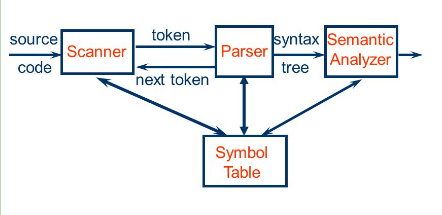
\includegraphics[width=\linewidth]{scanparse.png}
	\caption{Scanning and parsing of code lines.}
	\label{fig:scanparse}
\end{figure}
In our case,we have scanned the code lines using regex library in python for all
types of statements available in the language which we designed according to the
syntax so defined for each.For a given programming statement, it firts tokenizes and
checks against all defined regexes.Defition of some regexes can be seen in the table
below.
\begin{table}
\begin{tabular}{ ||c | c|| }
\hline
Operation & Regex Definition     \\
\hline \hline
Addition &   \textbackslash{}s*( \textbackslash{}w+) \textbackslash{}s*= \textbackslash{}s*( \textbackslash{}w+) \textbackslash{}s* \textbackslash{}+ \textbackslash{}s*( \textbackslash{}w+) \textbackslash{}s*  \\
\hline
Extern &Variable extern \textbackslash{}s+( \textbackslash{}w+) \textbackslash{}s*   \\
\hline
Loop & \textbackslash{}s*loop \textbackslash{}s+( \textbackslash{}w+) \textbackslash{}s*    \\
\hline
Macro & \textbackslash{}s*macro \textbackslash{}s*    \\
\hline
Minimum of a list &  \\
e.g., min(2,3,0,1) &  \textbackslash{}s*( \textbackslash{}w+) \textbackslash{}s*= \textbackslash{}s*min \textbackslash{}s* \textbackslash{}((.*) \textbackslash{}) \textbackslash{}s*    \textbackslash{}	\\
\hline
\end{tabular}
\caption{Some regex definitions in python.}
\label{regex_eq}
\end{table}
One of the most important uses of the theory of formal languages is in the definition
of programming languages and in the construction of interpreters and compilers
for them. The basic problem here is to define a programming language precisely and
to use this definition as the starting point for the writing of efficient and reliable
translation programs. Both regular and context-free languages are important in
achieving this. As we have seen, regular languages are used in the recognition of
certain simple patterns that occur in programming languages, but as we argue in
the introduction to this chapter, we need context-free languages to model more complicated
aspects.\newline
As with most other languages, we can define a programming language by a grammar.\newline
It is traditional in writing on programming languages to use a convention for
specifying grammars called the Backus-Naur form or BNF. This form is in essence
the same as the notation we have used here, but the appearance is different. In
BNF, variables are enclosed in triangular brackets. Terminal symbols are written
without any special marking. BNF also uses subsidiary symbols such as |, much in
the way we have done.\newline
Many parts of C-like programming languages are susceptible to definition by restricted
forms of context-free grammars. For example, the while statement in C can
be defined as Here the keyword while is a terminal symbol. All other terms are
variables, which still have to be defined.\newline
Unfortunately, not all features of a typical programming language can be expressed
by an s- grammar. The rules for above are not of this type, so that parsing becomes
less obvious. The question then arises what grammatical rules we can permit and
still parse efficiently. In compilers, extensive use has been made of what are called
LL and LR grammars. These grammars have the ability to express the less obvious
features of a programming language, yet allow us to parse in linear time.\newline
In connection with this, the issue of ambiguity takes on added significance. The
specification of aprogramming language must be unambiguous, otherwise a program
may yield very different results when processed by different compilers or run
on different systems. As Example 5.11 shows, a naive approach can easily introduce
ambiguity in the grammar. To avoid such mistakes we must be able to recognize
and remove ambiguities. A related question is whether a language is or is not inherently
ambiguous. What we need for this purpose are algorithms for detecting and
removing ambiguities in context-free grammars and for deciding whether or not a
context-free language is inherently ambiguous. Unfortunately, these are very diffi-
cult tasks, impossible in the most general sense, as we will see later.\newline
Those aspects of a programming language that can be modeled by a context-free
grammar are usually referred to as its syntax. However, it is normally the case that
not all programs that are syntactically correct in this sense are in fact acceptable
programs. For C, the usual BNF definition allows constructs such as\newline
char a, b, c; followed by\newline
c = 3.2;\newline
This combination is not acceptable to C compilers since it violates the constraint, “a
character variable cannot be assigned a real value.” Context-free grammars cannot
express the fact that type clashes may not be permitted. Such rules are part of
programming language semantics, since they have to do with how we interpret the
meaning of a particular construct. Programming language semantics are a complicated
matter. Nothing as elegant and concise as context-free grammars exists for
the specification of programming language semantics, and consequently some semantic
features may be poorly defined or ambiguous. It is an ongoing concern both
in programming languages and in formal language theory to find effective methods
for defining programming language semantics. Several methods have been proposed,
but none of them has been as universally accepted and are as successful for semantic
definition as context-free languages have been for syntax.
	\pagebreak
	\section{Assembler}
	\label{sec:assembler}
	\subsection{What is an assembler?}
	An assembler is a type of computer program that interprets software programs written in assembly language into machine language, code and instructions that can be executed by a computer. It serves as the bridge between symbolically coded instructions written in assembly language and the computer processor, memory and other computational components.\newline An assembler works by assembling and converting the source code of assembly language into object code or an object file that constitutes a stream of zeros and ones of machine code, which are directly executable by the processor. Assemblers are classified based on the number of times it takes them to read the source code before translating it; there are both single-pass and multi-pass assemblers. Moreover, some high-end assemblers provide enhanced functionality by enabling the use of control statements, data abstraction services and providing support for object-oriented programming structures. It enables software and application developers to access, operate and manage a computer's hardware architecture and components. It is sometimes referred to as the compiler of assembly language. It also provides the services of an interpreter.
	\subsection{Data Structure}
	\begin{itemize}
		\item Op code table (OPTAB) \newline
		It is used to look up mnemonic operation codes and translate them to their machine language equivalents. It is usually organized as a hash table, with mnemonic operation code as the key. The hash table organization is particularly appropriate, since it provides fast retrieval with a minimum of searching. In most cases, OPTAB is a static table – that is, entries are not normally added to or deleted from it. In such cases it is possible to design a special hashing function or other data structure to give optimum performance for the particular set of keys being stored. Most of the time, however, a general –purpose hashing method is used. 
		\item Symbol Table (SYMTAB) \newline
		It includes the name and value (address) for each label in the source program, together with flags to indicate error conditions (e.g,. a symbol defined in two different places). This table may also contain other information about the data area or instruction labeled – for example, its type or length. During Pass 1 of the assembler, labels are entered into SYMTAB as they are encounterd in the source program, along with their assigned addresses (from LOCCTR). During Pass 2, symbols used as operands are looked up in SYMTAB to obtain the addresses to be inserted in the assembled intructions. It is usually organized as a hash table for efficiency or insertion and retrieval. Since entries are rarely deleted from this table, efficiency of deletion is not an important consideration. Because SYMTAB is used havily throughout the assemble, similar characteristics – for example, labels that start or end with the same characters (like LOOP1, LOOP2 ) or are of the same length. It is important that the hashing fuction used perform well with such no-random keys. Division of the entire key by a prime table length often gives good result. 
		\item Location Counter (LOCCTR) \newline
		This is a variable that is used to help in the assignment of addresses. LOCCTR is initialized to the beginning address specified in the START statement. After each source statement is processed, the length of the assembled instructions or date area to be generated is added to LOCCTR. Thus whenever we reach a label in the source program, the current value of LOCCTR gives the address to be associated with that label. 
	\end{itemize}
	\subsection{Pass 1 Assembler}
	A single pass assembler scans the program only once and creates the equivalent binary program. It substitutes all of the symbolic instruction with machine code in one pass. The reason of using single pass assemblers is:
	\begin{itemize}
		\item It is necessary or desirable to avoid a second pass over the source program.
		\item The external storage for the intermediate file between two passes is slow or is inconvenient to use.
	\end{itemize}
	Algorithm for pass 1 assembler is given below: \newline
	Loop until the end of the program
	\begin{enumerate}
		\item Read in a line of assembly code
		\item Assign an address to this line
		\begin{itemize}
			\item Increment N (word addressing or byte addressing)
		\end{itemize}
		\item Save address values assigned to labels
		\begin{itemize}
			\item In symbol tables
		\end{itemize}
		\item Process assembler directives
		\begin{itemize}
			\item Constant declaration
			\item Space reservation
		\end{itemize}
	\end{enumerate}
	Following is the pseudocode of pass 1 asembler
	\begin{verbatim}
	begin
	  if starting address is given
	    LOCCTR = starting address;
	  else
	    LOCCTR = 0;
	  while OPCODE != END do                 ;; or EOF
	  begin
	    read a line from the code
	    if there is a label
  	      if this label is in SYMTAB, then error
	    else insert (label, LOCCTR) into SYMTAB
	    search OPTAB for the op code
	    if found
	      LOCCTR += N           ;; N is the length of this instruction (4 for MIPS)
	    else if this is an assembly directive
	    update LOCCTR as directed
	    else error
	    write line to intermediate file
	  end
	  program size =  LOCCTR - starting address;
	end
	\end{verbatim}
	After Pass 1 and before Pass 1 codes are displayed below:
	\begin{verbatim}
	var a = 0
	loop 3
	a = a + 1
	endloop
	\end{verbatim}
	Assembly code produced is:
		\begin{verbatim}
	MVI D, =’0’
	MOV #a,D
	PUSH E
	MVI E, 3
	LDA #a
	ADI 1
	STA #a
	MOV A,E
	SUI 1
	MOV E,A
	JNZ loop0
	POP E
	END
	a DS 1
	=’0’\end{verbatim}
	The symbols table and literals table are shown below:
	\newline
	Symbols Table
	\begin{verbatim}
	a : #23
	loop : %6
	\end{verbatim}
	Literals Table
	\begin{verbatim}
	0: 24
	\end{verbatim}
	\subsection{Pass 2 Assembler}
	Two pass translation of an assembly language program can handle forward references
	easily. LC processing is performed in the first pass and symbols defined in the program
	are entered into the symbol table. The second pass synthesizes the target form
	using the address information found in the symbol table. In effect, the first pass
	performs the analysis of the source program while the second pass performs synthesis
	of target program. The first pass constructs an intermediate representation (IR)
	of the source program for use by the second pass.\newline
	Consider an assembler instruction like the following:-
	\begin{verbatim}
	JMP LATER
	...
	...
	LATER:
	\end{verbatim}
	This is known as a forward reference. If the assembler is processing the file one
	line at a time, then it doesn’t know where LATER is when it first encounters the
	jump instruction. So, it doesn’t know if the jump is a short jump, a near jump or
	a far jump. There is a large difference amongst these instructions. They are 2, 3,
	and 5 bytes long respectively. The assembler would have to guess how far away the instruction is in order to generate the correct instruction. If the assembler guesses
	wrong, then the addresses for all other labels later in the program woulds be wrong,
	and the code would have to be regenerated. Or, the assembler could alway choose
	the worst case. But this would mean generating inefficiency in the program, since
	all jumps would be considered far jumps and would be 5 bytes long, where actually
	most jumps are short jumps, which are only 2 bytes long.\newline
	So, what is to be done to allow the assembler to generate the correct instruction?
	Answer: scan the code twice. The first time, just count how long the machine code
	instructions will be, just to find out the addresses of all the labels. Also, create a
	table that has a list of all the addresses and where they will be in the program.
	This table is known as the symbol table. On the second scan, generate the machine
	code, and use the symbol table to determine how far away jump labels are, and to
	generate the most efficient instruction.\newline
	This is known as a two-pass assembler. Each pass scans the program, the first
	pass generates the symbol table and the second pass generates the machine code.\newline
	The two pass assembler performs two passes over the source program.\newline
	In the first pass, it reads the entire source program, looking only for label definitions.
	All the labels are collected, assigned address, and placed in the symbol
	table in this pass, no instructions as assembled and at the end the symbol table
	should contain all the labels defined in the program. To assign address to labels,
	the assembles maintains a Location Counter (LC).\newline 
	In the second pass the instructions are again read and are assembled using the
	symbol table. Basically, the assembler goes through the program one line at a time,
	and generates machine code for that instruction. Then the assembler proceeds to the
	next instruction. In this way, the entire machine code program is created. For most
	instructions this process works fine, for example for instructions that only reference
	registers, the assembler can compute the machine code easily, since the assembler
	knows where the registers are.\newline
	Algorithm of Pass 2 Assembler is given below: \newline
	Loop until the end of the program
	\begin{enumerate}
		\item Read in a line of assembly code
		\item Assign an address to this line
		\begin{itemize}
			\item Increment N (word addressing or byte addressing)
		\end{itemize}
		\item Save address values assigned to labels
		\begin{itemize}
			\item In symbol tables
		\end{itemize}
		\item Process assembler directives
		\begin{itemize}
			\item Constant declaration
			\item Space reservation
		\end{itemize}
	\end{enumerate}
	Once Again perform the loop until the end of the program
	\begin{enumerate}
		\item Read in a line of code
		\item Translate opcode using opcode table
		\item Change labels to address using the symbol table
		\item Process assembler directives
		\item Produce object program
	\end{enumerate}
	\subsection{Difference between Pass 1 and Pass 2 Assembler}
The difference between one pass and two pass assemblers are:-\newline
A one pass assembler passes over the source file exactly once, in the same pass
collecting the labels, resolving future references and doing the actual assembly. The
difficult part is to resolve future label references (the problem of forward referencing)
and assemble code in one pass. The one pass assembler prepares an intermediate
file, which is used as input by the two pass assembler.\newline
A two pass assembler does two passes over the source file (the second pass can be
over an intermediate file generated in the first pass of the assembler). In the first
pass all it does is looks for label definitions and introduces them in the symbol table
(a dynamic table which includes the label name and address for each label in the
source program). In the second pass, after the symbol table is complete, it does the
actual assembly by translating the operations into machine codes and so on.
	\pagebreak
	\section{Linker}
	\subsection{What is a Linker?}
	In high level languages, some built in header files or libraries are stored. These
	libraries are predefined and these contain basic functions which are essential for executing
	the program. These functions are linked to the libraries by a program called
	Linker. If linker does not find a library of a function then it informs to compiler and
	then compiler generates an error. The compiler automatically invokes the linker as
	the last step in compiling a program.\newline
	Computer programs typically are composed of several parts or modules; these parts/modules
	need not all be contained within a single object file, and in such cases refer to each
	other by means of symbols. Typically, an object file can contain three kinds of
	symbols:
	\begin{itemize}
		\item defined "external" symbols, sometimes called "public" or "entry" symbols, which allow it to be called by other modules.
		\item undefined "external" symbols, which reference other modules where these symbols are defined.
		\item local symbols, used internally within the object file to facilitate relocation.
	\end{itemize}

	For most compilers, each object file is the result of compiling one input source code
	file. When a program comprises multiple object files, the linker combines these files
	into a unified executable program, resolving the symbols as it goes along.
	Linkers can take objects from a collection called a library. Some linkers do not
	include the whole library in the output; they include only its symbols that are referenced
	from other object files or libraries. Libraries exist for diverse purposes, and
	one or more system libraries are usually linked in by default.
	The linker also takes care of arranging the objects in a program’s address space.
	This may involve relocating code that assumes a specific base address to another
	base. Since a compiler seldom knows where an object will reside, it often assumes
	a fixed base location (for example, zero). Relocating machine code may involve retargeting
	of absolute jumps, loads and stores.
	The executable output by the linker may need another relocation pass when it is
	finally loaded into memory (just before execution). This pass is usually omitted on
	hardware offering virtual memory: every program is put into its own address space,
	so there is no conflict even if all programs load at the same base address. This pass
	may also be omitted if the executable is a position independent executable.
	Not built in libraries, it also links the user defined functions to the user defined
	libraries. Usually a longer program is divided into smaller subprograms called modules.
	And these modules must be combined to execute the program. The process of
	combining the modules is done by the linker.
	\subsection{Tasks of a Linker}
	\begin{itemize}
		\item Searches the program to find library routines used by program, e.g. printf(),
		math routines.
		\item Determines the memory locations that code from each module will occupy and
		relocates its instructions by adjusting absolute references.
		\item Resolves references among files
	\end{itemize}
    \subsection{Linking Requirements}
\begin{itemize}
	\item All program units are translated separately.
	\item Hence, all sub program calls and common variable reference require linking.
	\item Programs are nested in main program.
	\item Procedure reference do not require linking, they can be handled using relocation.
	\item Build in functions require linking.
	\item Linker processes all object modules being linked and builds a table of all public definition and load time address.
	\item Name Table (NTAB)
	\begin{itemize}
		\item Symbol : Symbol Name for external reference or object module.
		\item Linked Address : For public definition contains link-address. For object module contains link-origin.
	\end{itemize}
	\item Most information in NTAB is derived from LINKTAB entries with type=PD.
\end{itemize}
\subsection{Algorithm of a Linker}
\begin{enumerate}
	\item program-linked-origin:= <link origin> from linker command.
	\item For each object module
	\begin{itemize}
		\item t-origin:= translated origin of object module. OM-size:=size of the object module;
		\item Relocation-factor:= program-linked-origin–t-origin.
		\item Read the machine language program in work-area .
		\item Read LINKTAB of the object module.
		\item For each LINKTAB entry with type = PD\newline
		name:= symbol;\newline
		linked-address := translated-address + relocation-factor;\newline
		enter(name,linked-address) in NTAB.\newline
		\item Enter (object module name, program-linked-origin ) in NTAB;
		\item program-linked-origin := program-linked-origin + OM-size ;
	\end{itemize}
	\item for each object module
	\begin{itemize}
		\item t-origin := translated origin of the object module.
		\item For each LINKTAB entry with type=EXT
		\begin{itemize} 
			\item address-in-work-area := address of work-area + program-linked-origin
			\item < link-origin > + translated address \item ‘ t-origin ;
			\item Search symbol in NTAB and copy its linked address. Add the linked address to the operand address in the word with the address addressin-work-area.
		\end{itemize}
	\end{itemize}
\end{enumerate}
Example\newline
\begin{table}\centering
	\begin{tabular}{ ||c|c||}
		\hline \hline
		Symbol & Linked Address \\
	\hline	\hline
		P      & 900            \\
	\hline	
	A      & 940            \\
	\hline
		Q      & 942            \\
	\hline	
	Alpha  & 973     \\
	\hline      
	\end{tabular}
	\caption{NTAB Information}
	\label{ntab_info}
\end{table}

\begin{itemize}
	\item While linking program P and program Q with linked-origin =900, NTAB contains above information:
	\item Work-area = 300.
	\item When LINKTAB of alpha is processed during linking, address-in-work-area := 300 + 900 - 900 + 518 – 500. i.e 318.
	\item Hence linked address of ALPHA is 973, is copied from NTAB entry of ALPHA and added to word in address 318.
\end{itemize}
\subsection{Relocation}
As the compiler has no information on the layout of objects in the final output, it cannot take advantage of shorter or more efficient instructions that place a requirement on the address of another object. For example, a jump instruction can reference an absolute address or an offset from the current location, and the offset could be expressed with different lengths depending on the distance to the target.\newline
By generating the most conservative instruction (usually the largest relative or absolute variant, depending on platform) and adding relaxation hints, it is possible to substitute shorter or more efficient instructions during the final link. This step can be performed only after all input objects have been read and assigned temporary addresses; the linker relaxation pass subsequently reassigns addresses, which may in turn allow more relaxations to occur. In general, the substituted sequences are shorter, which allows this process to always converge on the best solution given a fixed order of objects; if this is not the case, relaxations can conflict, and the linker needs to weigh the advantages of either option.\newline
While instruction relaxation typically occurs at link-time, inner-module relaxation can already take place as part of the optimising process at compile-time. In some cases, relaxation can also occur at load-time as part of the relocation process or combined with dynamic dead-code elimination techniques. Consider a program consisting of 2 different files and one of them having extern variable to use variable of another file.\newline
First file contains:\newline
global a = 5\newline
While 2nd file contains\newline
extern a\newline
a = a + 2\newline
Output given by linker:\newline
\begin{verbatim}
MVI D, ='5'
MOV @A,D
END
a DS 1
='5'
LDA @4
ADI 2
STA @4
END
\end{verbatim}

	\section{Loader}
	\subsection{What is a Loader?}
	Loader is a program that loads machine codes of a program into the system memory.
	In Computing, a loader is the part of an Operating System that is responsible
	for loading programs. It is one of the essential stages in the process of starting a
	program. Because it places programs into memory and prepares them for execution.
	Loading a program involves reading the contents of executable file into memory.
	Once loading is complete, the operating system starts the program by passing
	control to the loaded program code. All operating systems that support program
	loading have loaders. In many operating systems the loader is permanently resident
	in memory.
	In computer systems a loader is the part of an operating system that is responsible
	for loading programs and libraries. It is one of the essential stages in the process
	of starting a program, as it places programs into memory and prepares them for
	execution. Loading a program involves reading the contents of the executable file
	containing the program instructions into memory, and then carrying out other required
	preparatory tasks to prepare the executable for running. Once loading is
	complete, the operating system starts the program by passing control to the loaded
	program code.
	All operating systems that support program loading have loaders, apart from highly
	specialized computer systems that only have a fixed set of specialized programs.
	Embedded systems typically do not have loaders, and instead the code executes
	directly from ROM. In order to load the operating system itself, as part of booting,
	a specialized boot loader is used. In many operating systems the loader is permanently
	resident in memory, although some operating systems that support virtual
	memory may allow the loader to be located in a region of memory that is pageable.
	In the case of operating systems that support virtual memory, the loader may not
	actually copy the contents of executable files into memory, but rather may simply
	declare to the virtual memory subsystem that there is a mapping between a region
	of memory allocated to contain the running program’s code and the contents of the
	associated executable file. (See memory-mapped file.) The virtual memory subsystem
	is then made aware that pages with that region of memory need to be filled on
	demand if and when program execution actually hits those areas of unfilled memory.
	This may mean parts of a program’s code are not actually copied into memory until
	they are actually used, and unused code may never be loaded into memory at all.
	It is the part of the OS that brings an executable file residing on disk into memory
	and starts it running.
	The main task of the loader is to bring binary executable image into main memory
	and bind the relocatable addresses into absolute addresses.
	\newline\newline
	The binary image of a program consists of following parts :-
	\begin{itemize}
		\item  Header – It shows the type of file (executable or library file).
		\item  Text – It shows the actual code of the program
		\item  List of shared libraries - libraries that have been used in the object file.
	\end{itemize}
\begin{figure}[h!]
	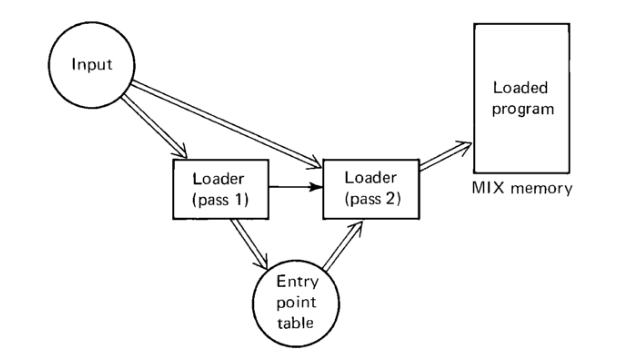
\includegraphics[width=\linewidth]{loader.png}
	\caption{Functioning of a Loader}
	\label{fig:loader}
\end{figure}
	\subsection{Execution of Loader}
	The steps on how loading is executed are shown below:
	\begin{itemize}
		\item Read executable file’s header to determine the size of text and data segments.
		\item Create a new address space for the program.
		\item Copies instructions and data into address space.
		\item Copies arguments passed to the program on the stack.
		\item Initializes the machine registers including the stack ptr.
		\item Jumps to a startup routine that copies the program’s arguments from the stack to registers and calls the program’s main routine
	\end{itemize}

	\subsection{Design of an absolute Loader}
	An absolute object file consists of three parts
	\begin{enumerate}
	\item The start address of the program
	\item The object instructions
	\item The address of the first executable instruction. This is placed in the object
	file by assembler in response to the END directive. It is either the address
	specified by the END or, in the absence of such an address is identical to the
	first address of the program.
	\end{enumerate}
	The loader reads the first item and loads the rest of object file into successive memory
	locations.
	\pagebreak

	\section{Refrences}
	\begin{itemize}
\item Systems Programming and Operating Systems by Dhananjay Dhamdhere 
\item 2-pass Assembler explanation
 \item wiki-assembler
 \item Linker and Loader by John R. Levine
	\end{itemize}
	\pagebreak
	
\end{document}